% This is a Basic Assignment Paper but with like Code and stuff allowed in it, there is also url, hyperlinks from contents included. 

\documentclass[11pt]{article}

% Preamble

\usepackage[margin=1in]{geometry}
\usepackage{amsfonts, amsmath, amssymb}
\usepackage{fancyhdr, float, graphicx}
\usepackage[utf8]{inputenc} % Required for inputting international characters
\usepackage[T1]{fontenc} % Output font encoding for international characters
\usepackage{fouriernc} % Use the New Century Schoolbook font
\usepackage[nottoc, notlot, notlof]{tocbibind}
\usepackage{listings}
\usepackage{xcolor}
\usepackage{blindtext}
\usepackage{hyperref}
\hypersetup{
    colorlinks=true,
    linkcolor=black,
    filecolor=magenta,      
    urlcolor=cyan,
    pdfpagemode=FullScreen,
    }

\definecolor{codegreen}{rgb}{0,0.6,0}
\definecolor{codegray}{rgb}{0.5,0.5,0.5}
\definecolor{codepurple}{rgb}{0.58,0,0.82}
\definecolor{backcolour}{rgb}{0.95,0.95,0.92}

\lstdefinestyle{mystyle}{
    backgroundcolor=\color{backcolour},   
    commentstyle=\color{codegreen},
    keywordstyle=\color{magenta},
    numberstyle=\tiny\color{codegray},
    stringstyle=\color{codepurple},
    basicstyle=\ttfamily\footnotesize,
    breakatwhitespace=false,         
    breaklines=true,                 
    captionpos=b,                    
    keepspaces=true,                 
    numbers=left,                    
    numbersep=5pt,                  
    showspaces=false,                
    showstringspaces=false,
    showtabs=false,                  
    tabsize=2
}

\lstset{style=mystyle}

% Header and Footer
\pagestyle{fancy}
\fancyhead{}
\fancyfoot{}
\fancyhead[L]{\textit{\Large{Information and Cycbersecurity - 2nd Year B. Tech}}}
%\fancyhead[R]{\textit{something}}
\fancyfoot[C]{\thepage}
\renewcommand{\footrulewidth}{1pt}



% Other Doc Editing
% \parindent 0ex
%\renewcommand{\baselinestretch}{1.5}

\begin{document}

\begin{titlepage}
    \centering

    %---------------------------NAMES-------------------------------

    \huge\textsc{
        MIT World Peace University
    }\\

    \vspace{0.75\baselineskip} % space after Uni Name

    \LARGE{
        Information and Cybersecurity\\
        Second Year B. Tech, Semester 1
    }

    \vfill % space after Sub Name

    %--------------------------TITLE-------------------------------

    \rule{\textwidth}{1.6pt}\vspace*{-\baselineskip}\vspace*{2pt}
    \rule{\textwidth}{0.6pt}
    \vspace{0.75\baselineskip} % Whitespace above the title



    \huge{\textsc{
            Secured web applications
        }} \\



    \vspace{0.5\baselineskip} % Whitespace below the title
    \rule{\textwidth}{0.6pt}\vspace*{-\baselineskip}\vspace*{2.8pt}
    \rule{\textwidth}{1.6pt}

    \vspace{1\baselineskip} % Whitespace after the title block

    %--------------------------SUBTITLE --------------------------	

    \LARGE\textsc{
        Lab Assignment 9
    } % Subtitle or further description
    \vfill

    %--------------------------AUTHOR-------------------------------

    Prepared By
    \vspace{0.5\baselineskip} % Whitespace before the editors

    \Large{
        Krishnaraj Thadesar \\
        Cyber Security and Forensics\\
        Batch A1, PA 20
    }


    \vspace{0.5\baselineskip} % Whitespace below the editor list
    \today

\end{titlepage}


\tableofcontents
\thispagestyle{empty}
\clearpage

\setcounter{page}{1}

\section{Aim}

Demonstration of secured web applications system using SSL certificates and its
deployment in Apache tomcat server

\section{Objectives}
To learn different vulnerability scanning.

\section{Theory}

\subsection{SSL Certificate}
An SSL (Secure Sockets Layer) certificate is a digital certificate that verifies the authenticity of a website and encrypts data transmitted between the website and the user's web browser. SSL certificates ensure that all sensitive information, such as usernames, passwords, and credit card numbers, are transmitted securely over the internet.

\subsection{How does an SSL certificate work?}
When a user visits a website that has an SSL certificate, the website's server sends the user's web browser a copy of the certificate. The browser then verifies the certificate with the Certificate Authority (CA) that issued it. If the certificate is valid, the browser establishes a secure connection with the website using SSL/TLS encryption.

\subsection{Types of SSL certificates}
There are different types of SSL certificates based on the number of domains or subdomains they cover, the level of validation, and the warranty offered by the Certificate Authority (CA). Some common types of SSL certificates include:

\begin{enumerate}
    \item Domain Validated (DV) SSL Certificate: This type of SSL certificate only validates the domain name of the website, ensuring that it belongs to the entity requesting the certificate. DV SSL certificates are the most common type of SSL certificate and are suitable for personal websites or blogs.
    \item Organization Validated (OV) SSL Certificate: This type of SSL certificate validates both the domain name and the identity of the organization or business requesting the certificate. OV SSL certificates are suitable for e-commerce websites and other online businesses.
    \item Extended Validation (EV) SSL Certificate: This type of SSL certificate provides the highest level of validation and requires extensive documentation to prove the identity of the organization requesting the certificate. EV SSL certificates are suitable for large businesses and financial institutions.
    \item Wildcard SSL Certificate: This type of SSL certificate covers multiple subdomains of a single domain name. For example, a wildcard SSL certificate for the domain example.com would cover subdomains such as blog.example.com and shop.example.com.
\end{enumerate}

\subsection{Benefits of SSL certificates}

There are several benefits of using an SSL certificate for a website, including:
\begin{enumerate}
    \item Data encryption: SSL certificates encrypt all data transmitted between the website and the user's web browser, ensuring that sensitive information is secure.
    \item Authentication: SSL certificates provide authentication, verifying that the website is legitimate and belongs to the entity requesting the certificate.
    \item Trust and credibility: SSL certificates display trust indicators, such as the padlock icon in the web browser's address bar, which can increase a website's credibility and reputation.
    \item SEO benefits: SSL certificates can improve a website's search engine ranking, as search engines prefer secure websites.
    \item

\end{enumerate}
\subsection{Example}
Suppose you want to create an e-commerce website where users can purchase products and enter their personal information, such as name, address, and credit card details. To ensure that the website is secure and trustworthy, you decide to obtain an SSL certificate.\\

You choose to purchase an OV SSL certificate, which will validate your domain name and your business's identity. You submit your company's legal documents and undergo a validation process to prove your identity.\\

Once the CA verifies your documents and identity, they issue the SSL certificate, which you install on your website's server. Now, when users visit your website, their web browsers will establish a secure connection using SSL/TLS encryption, ensuring that their personal information is protected.

\section{Platform}
\textbf{\textbf{Operating System}}: Arch Linux x86-64 \\
\textbf{\textbf{IDEs or Text Editors Used}}: Visual Studio Code\\

\section{Input and Output}
\begin{figure}[H]
    \centering
    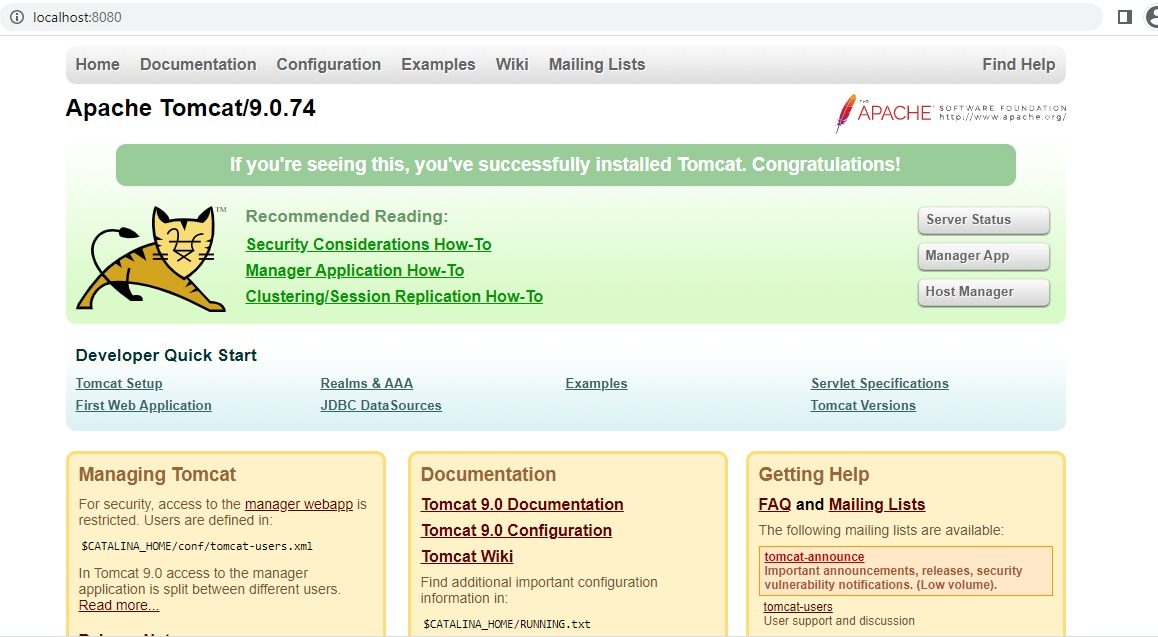
\includegraphics[width=.95\textwidth]{tomcat.jpeg}
    \caption{}
\end{figure}
\begin{figure}[H]
    \centering
    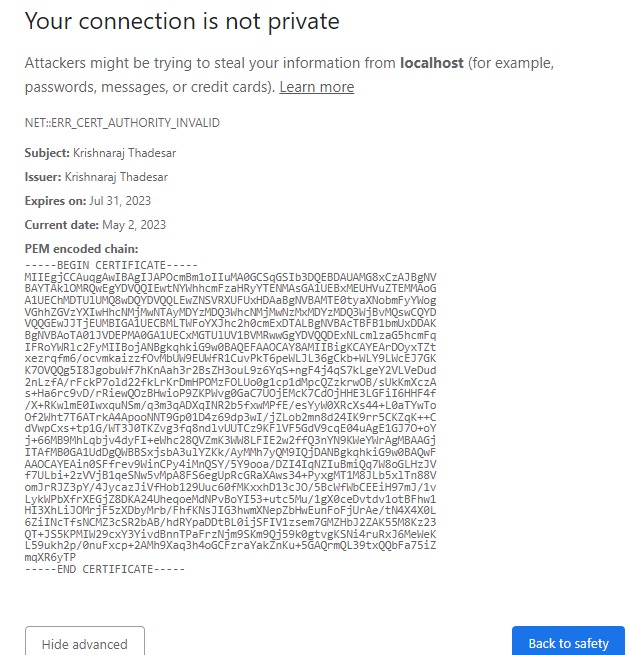
\includegraphics[width=.95\textwidth]{tomcat1.jpeg}
    \caption{}
\end{figure}
\begin{figure}[H]
    \centering
    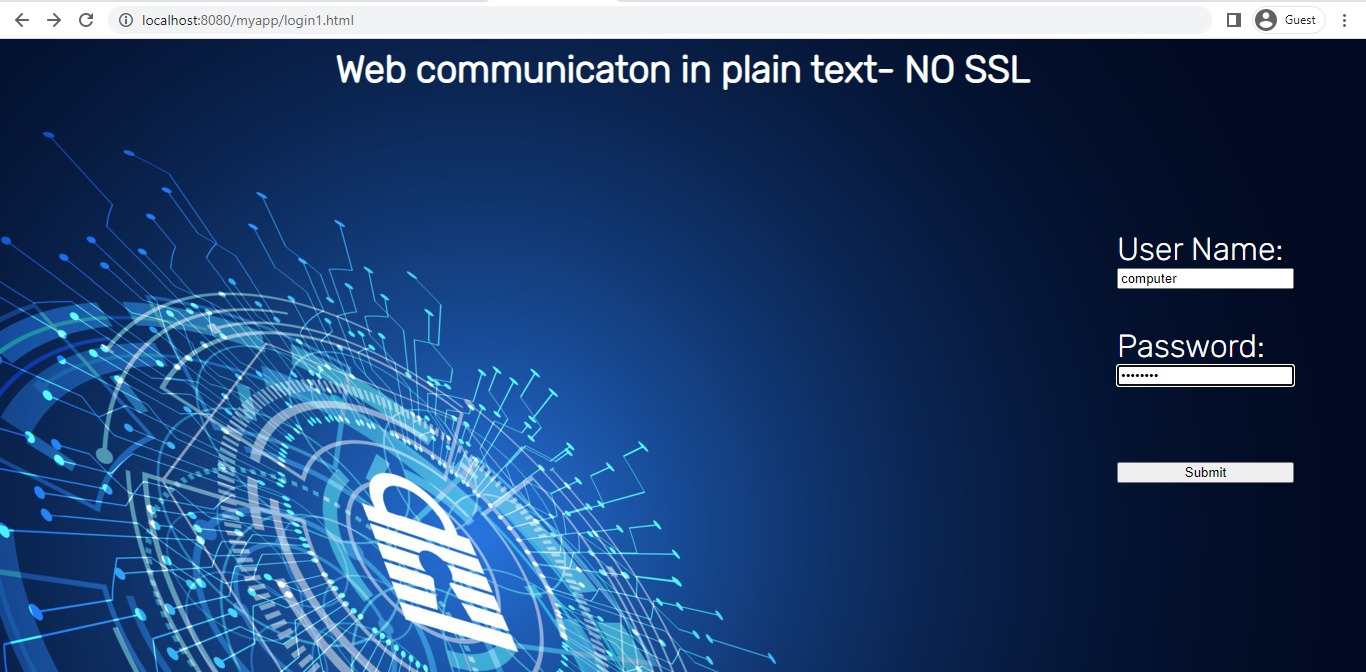
\includegraphics[width=.95\textwidth]{tomcat2.jpeg}
    \caption{}
\end{figure}
\begin{figure}[H]
    \centering
    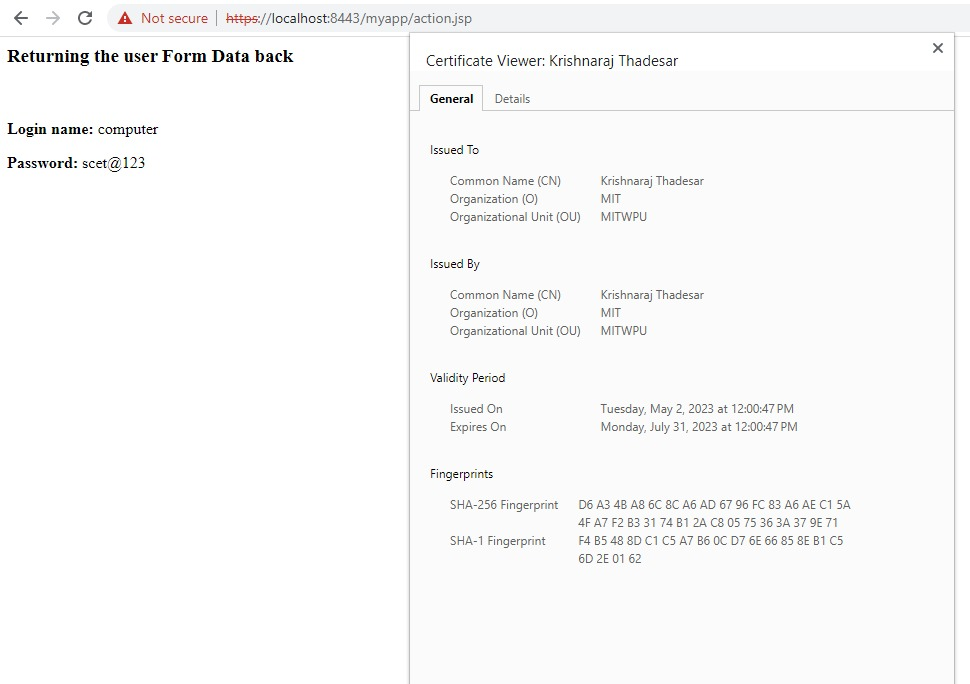
\includegraphics[width=.95\textwidth]{tomcat3.jpeg}
    \caption{}
\end{figure}
\begin{verbatim}
The Given Signature is Valid
\end{verbatim}


% \section{Code}
% \lstinputlisting[language=Python, caption="DSA Signature Validity using PyCrypto Library"]{../Programs/Assignment_7/dsa using lib.py}

\section{Conclusion}
Thus, we have successfully implemented
\clearpage

\section{FAQ}

\begin{enumerate}
    \item \textbf{What type of encryption does SSL use?}\\

          Secure Socket Layer (SSL) uses a combination of symmetric and asymmetric encryption to secure data transmitted over a network. SSL uses asymmetric encryption during the initial handshake process, where the client and server exchange public keys to establish a secure communication channel. Once the secure channel is established, SSL uses symmetric encryption to encrypt the data being transmitted between the client and server.\\

          Symmetric encryption uses a single secret key to encrypt and decrypt data, while asymmetric encryption uses a pair of keys, one private and one public. The public key can be freely shared, while the private key is kept secret. In SSL, the public key is used to encrypt the data, and the private key is used to decrypt the data.\\

          SSL supports a variety of symmetric encryption algorithms, including AES, DES, and 3DES. It also supports a variety of asymmetric encryption algorithms, including RSA, DSA, and ECDSA.

    \item \textbf{How safe is SSL?}\\

          SSL is generally considered to be a secure protocol for transmitting sensitive data over a network. SSL has undergone multiple revisions over the years, with the latest version being Transport Layer Security (TLS). TLS version 1.3 is the latest and most secure version of SSL/TLS, which has been designed to provide strong encryption and better security features.\\

          However, SSL can be vulnerable to various types of attacks, such as Man-in-the-Middle (MITM) attacks, where an attacker intercepts the communication between the client and server and eavesdrops on the conversation or alters the data being transmitted. SSL is also vulnerable to attacks that exploit weaknesses in the encryption algorithms or the SSL protocol itself.\\

          To mitigate these risks, SSL implementations must be properly configured and maintained to ensure they are up-to-date with the latest security patches and best practices. It is also recommended to use SSL/TLS certificates from trusted Certificate Authorities (CA) and to use strong passwords and multi-factor authentication to protect the private keys used for encryption.

    \item \textbf{What are the benefits of SSL?}\\

          The benefits of SSL include:

          \begin{enumerate}
              \item Data encryption: SSL encrypts the data transmitted between the client and server, which helps to protect the data from unauthorized access and eavesdropping.
              \item Authentication: SSL uses digital certificates to authenticate the identity of the server and ensure that the client is communicating with the intended server.
              \item Trust: SSL/TLS certificates are issued by trusted Certificate Authorities (CA) that verify the identity of the server and ensure that the SSL/TLS certificate is valid.
              \item Compliance: SSL is required by many industry regulations and compliance standards, such as the Payment Card Industry Data Security Standard (PCI DSS).
              \item Improved search engine ranking: Google has confirmed that HTTPS is a ranking factor, and using SSL/TLS can help to improve search engine rankings.
          \end{enumerate}

\end{enumerate}

\end{document}